\chapter{Semantics-First Approach to Clinical Decision Support}

In chapter \ref{chapter:introduction}, we explained that, despite
advances in medicine, mortality and costs associated with preventable
medical errors (\PMEs{}) remain unacceptably high. In chapter
\ref{chapter:background}, we explained how systems that
assist healthcare practitioners (\HCPs{}) with situation-specific
advice based on evidence-based best practice guidelines (\BPGs{}),
called clinical decision (\CDSSs{}) can reduce both mortality
and costs associated with \PMEs{}. But, despite their potential,
the uptake of such systems in practice is hindered by challenges
that were introduced in section \ref{sec:hurdles-cdss-adoption}, and
discussed in depth in chapter \ref{chapter:hurdles-cdss-adoption}.
In brief, the following challenges (Cs) were outlined:
\begin{enumerate}[label=C\arabic*.]
\itemsep0.0em
\item Absence of systematic ways of \emph{validating content}
in a \emph{reliable}, \emph{accessible} and \emph{updateable} manner.
\item Lack of \emph{reliable}, \emph{shareable} \CDSS{} content
that can be easily adopted across healthcare organizations and their (Information
Technology) \IT{} systems.
\item Technical difficulties of sharing due to \emph{need for
  adaptation} to diverse Electronic Health Records (\EHR) systems.
\item \emph{Suboptimal} User Interfaces (\UIs), implementation choices and
workflows.
\end{enumerate}

\begin{figure}[th!]
  \centering
  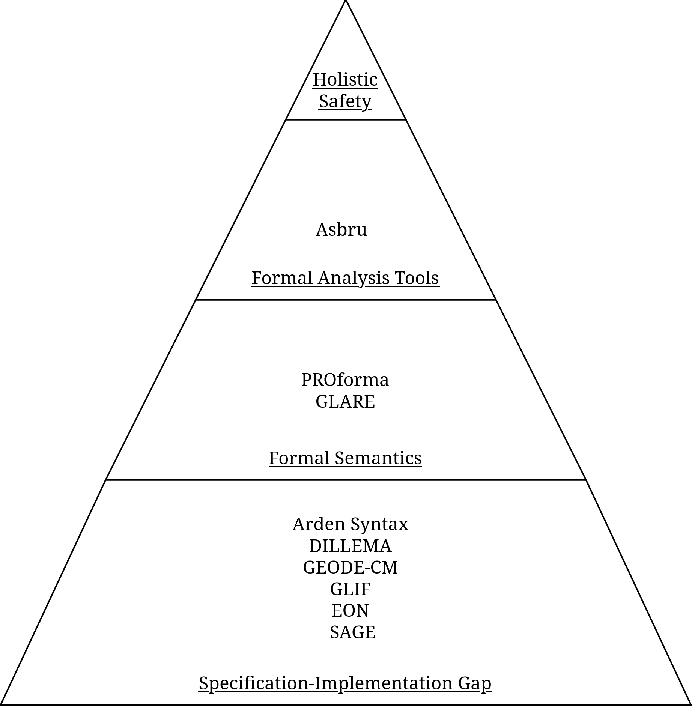
\includegraphics[width=0.5\textwidth]{pyramid}
  \caption{Existing \DSLs{} for Computer Interpretable Guidelines}\label{fig:existing-work-pyramid}
\end{figure}

Over the years, significant progress has been made towards
addressing these challenges. In chapter \ref{chapter:related-work},
we discussed how existing approaches have attempted to
address said challenges, and their limitations. Specifically,
in section \ref{sec:related-work-discussion}, we outlined major
themes that these approaches adopt to tackle these challenges.
This is further illustrated by the pyramid diagram in \figurename{}
\ref{fig:existing-work-pyramid}, where aforementioned themes are
underlined in the pyramid's various rungs.
As is typical, approaches that appear in higher rungs also
have characteristics of ones below them. For example, while guidelines expressed in
the Arden Syntax eliminate the specification-implementation gap by being
both \HCP{}-comprehensible and interpretable, they cannot be formally analyzed
due to lack of analysis tools in the ecosystem. Asbru-based guidelines
on the other hand not only eliminate the specification-implementation gap, but can also be
formally analyzed using support for KIV-based verification in the Asbru
ecosystem (see section \ref{sec:kiv-verification}).

As is evident in \figurename{} \ref{fig:existing-work-pyramid}, no
existing approach covers the \say{holistic safety} rung of the pyramid.
Recall from section \ref{sec:related-work-discussion} that we say an
approach tackles \say{holistic safety} if,
besides support for analyzing guidelines,
analysis and execution tools also have correctness guarantees.
In this work, we argue that such guarantees are necessary for
trustworthy \CDSSs{}. We attempt to address \say{holistic safety}
systematically by developing a \emph{semantics-first approach} for
building clinical decision support systems. In this context, by semantics-first
we mean that:
\begin{itemize}
  \item The semantics of the programming language for defining said knowledge is
    formally defined, from which execution and analysis tools are derived in a
    correct by construction manner, leading to holistic safety.
  \item The semantics of medical knowledge are expressed accurately.
\end{itemize}
At the core of our approach is a novel domain-specific language for expressing
medical knowledge called $\MediK{}$ (pronounced Medi-Kay). By being comprehensible to domain experts
in medicine, $\MediK{}$-based computer interpretable guidelines can serve
both as a guideline's non-executable \HCP{}-comprehensible description, i.e.,
the specification, and its encoding in a computable medium, i.e., the
implementation, thereby eliminating any specification-implementation gap.

The remainder of this chapter is structured as follows: Section
\ref{sec:semantics-first} briefly describes the semantics-first philosophy.
Next, Section \ref{sec:k-framework} describes $\K$ -- the language semantic
framework that $\MediK{}$'s are expressed in. Finally,
section \ref{sec:semantics-first-pitfalls} describes potential pitfalls
of following the semantics-first philosophy.

\section{Semantics-First Approach}\label{sec:semantics-first}

The semantics-first approach prescribes a systematic way of
developing programming languages. Instead of implementing
tools for a language, such as interpreters, compilers and
model checkers in ad-hoc manner, the approach states that the
first step in developing said tools must be to formally define
the language's semantics. As show in \figurename{} \ref{fig:semantics-first},
once defined, all tools for the language
can then be automatically derived from the semantics. Moreover, since
the tools utilize the semantics, they are, by definition,
correct-by-construction.

While following the semantics-first philosophy might seem like an obvious choice
in language design, its adoption in practice is far from ideal.
Conventional practice in the programming language and formal
methods community is still to develop analysis and execution tools for each
programming language from scratch \cite{ChenSETSS19}, as illustrated
in \figurename{} \ref{fig:conventional-pl-development} from
\cite{ChenSETSS19}. But, this approach has several
disadvantages:
\begin{itemize}
  \item Tools are often based on informal descriptions of language semantics,
    leaving developers to extrapolate finer details of the language's semantics,
    leading to inconsistencies.
    For instance, in \cite{ParkPLDI15}, it was found
    that ECMAScript 5.1-compliant JavaScript engines
    in mainstream web browsers exhibited different behaviors
    for certain complex JavaScript programs.
\end{itemize}

\begin{figure}[t!]
  \centering
  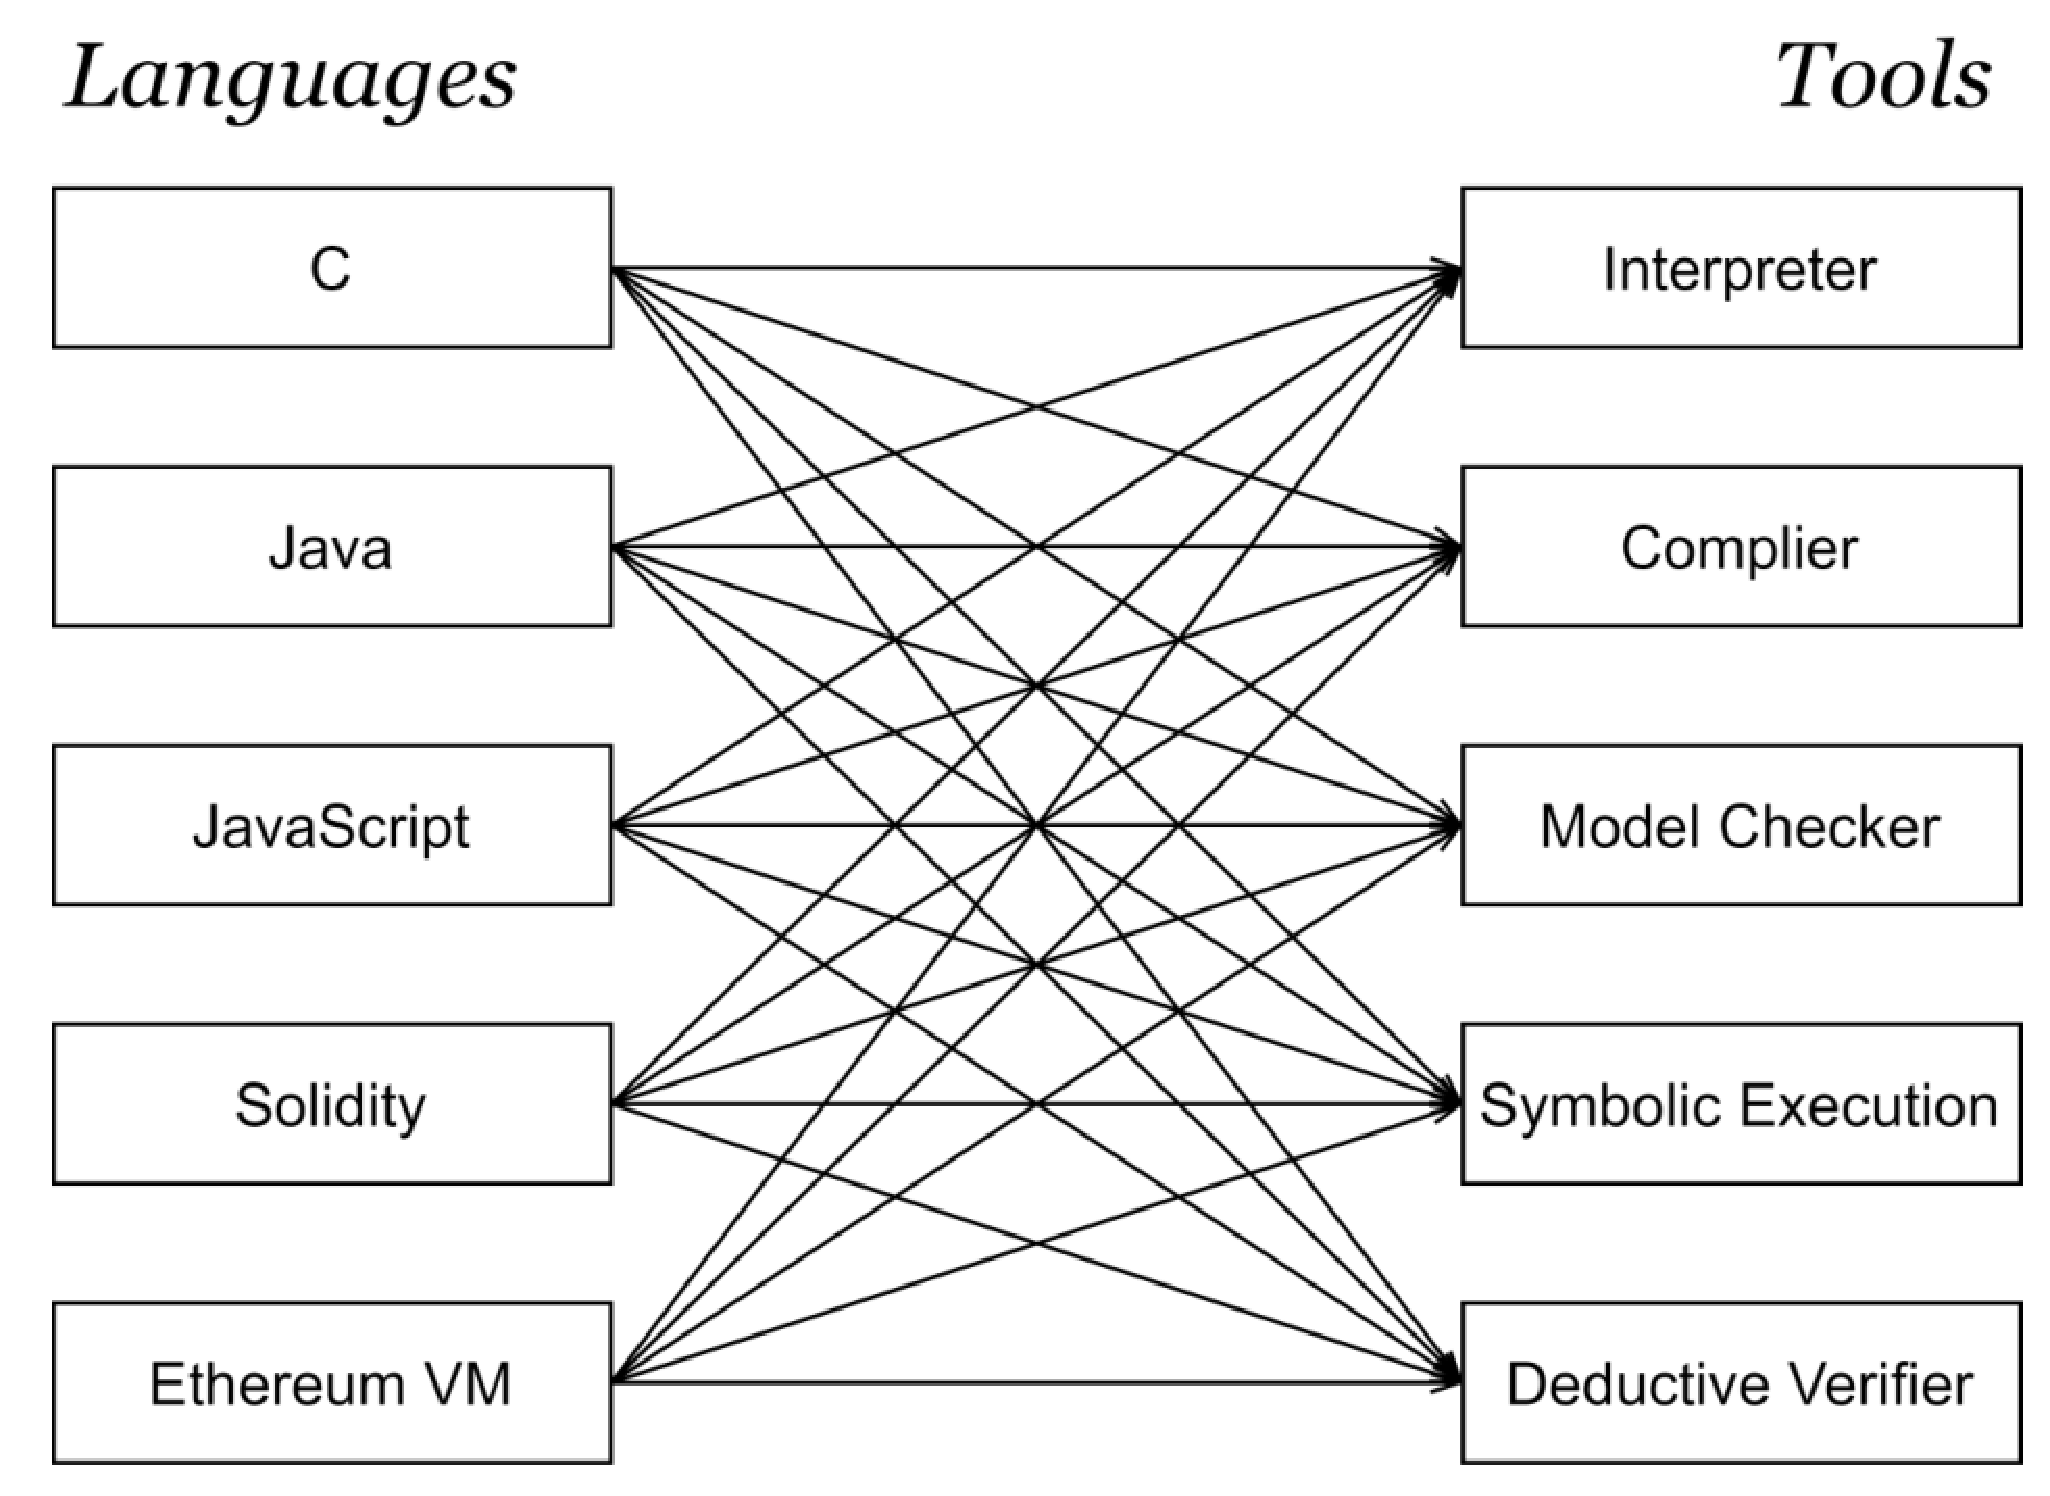
\includegraphics[width=0.6\textwidth]{conventional-pl-development}
  \caption{State-of-Art in Programming Language Design}\label{fig:conventional-pl-development}
\end{figure}

\section{The $\K{}$ Framework}\label{sec:k-framework}

\section{Pitfalls of the Semantics-First Approach}\label{sec:semantics-first-pitfalls}
